% Unit 121 terjemahan Bahasa Indonesia dari chapter9.tex baris 1--305.
% Sumber: Methods of Algebra, Volume 2, commit
% 9a5803ff77dd3257484cb177f851a73770a59dd3 (CC BY 4.0).
% stable-unit-id: o014.aljabr2.chapter9.duality-a
% Cakupan: pembukaan Bab 9 dan Bagian 9.1 sampai Definisi morfisme dual;
% Unit 122 berlanjut pada baris 306.

\hypertarget{o014.aljabr2.chapter9.duality-a}{ }
% segment-id: o014.aljabr2.chapter9.duality-a.h001
\chapter{Dualitas}\label{sec:duality}

% segment-id: o014.aljabr2.chapter9.duality-a.p001
Konsep dualitas berasal dari teori ruang vektor. Misalkan $\Bbbk$ suatu medan,
dan tuliskan ruang dual dari ruang vektor-$\Bbbk$ $V$ sebagai
$V^\vee:=\Hom_{\Bbbk}(V,\Bbbk)$. Terdapat
\begin{itemize}
	% segment-id: o014.aljabr2.chapter9.duality-a.i001
	\item pemetaan evaluasi $\mathrm{ev}:V\otimes V^\vee\to\Bbbk$, yang
	memetakan $v\otimes\lambda$ ke $\lambda(v)$;
	% segment-id: o014.aljabr2.chapter9.duality-a.i002
	\item jika $V$ berdimensi hingga, terdapat pula pemetaan koevaluasi
	$\mathrm{coev}:\Bbbk\to V^\vee\otimes V$, yang memetakan $1$ ke
	$\sum_{i=1}^n\check{v}_i\otimes v_i$, dengan $(v_i)_{i=1}^n$ sembarang basis
	dari $V$ dan $(\check{v}_i)_{i=1}^n$ basis dualnya.
\end{itemize}

% segment-id: o014.aljabr2.chapter9.duality-a.p002
Dalam kasus berdimensi hingga, keduanya memenuhi identitas dasar
% segment-id: o014.aljabr2.chapter9.duality-a.q001
\[ (\identity_{V^\vee} \otimes \mathrm{ev})(\mathrm{coev} \otimes \identity_{V^\vee}) = \identity_{V^\vee}, \quad (\mathrm{ev} \otimes \identity_V) (\identity_V \otimes \mathrm{coev}) = \identity_V. \]

% segment-id: o014.aljabr2.chapter9.duality-a.p003
Dalam kategori monoidal umum, data dual yang didefinisikan dalam
\S\ref{sec:monoidal-dual} merupakan generalisasi langsung dari situasi di
atas: data tersebut terdiri atas sepasang objek $(L,R)$ beserta morfisme
$\mathrm{ev}:L\otimes R\to\munit$ dan
$\mathrm{coev}:\munit\to R\otimes L$ yang memenuhi identitas dasar di atas.
Dalam keadaan ini, $R$ disebut dual kanan dari $L$, sedangkan $L$ disebut dual
kiri dari $R$. Kategori monoidal yang setiap objeknya memiliki dual kiri
(atau dual kanan) disebut kaku kiri (rigid kiri) atau kaku kanan (rigid
kanan), masing-masing.

% segment-id: o014.aljabr2.chapter9.duality-a.p004
Untuk kategori monoidal beranyam, \S\ref{sec:symm-monoidal-dual} akan
menjelaskan cara menghubungkan kedua jenis dual tersebut. Dengan demikian,
jika suatu objek $X$ memiliki dual, kita dapat mendefinisikan jejak
$\Tr(f)$ bagi $f\in\End(X)$ dan selanjutnya dimensi
$\dim X:=\Tr(\identity_X)$. Keduanya merupakan unsur $\End(\munit)$.
Tepatnya, masing-masing mempunyai versi kiri dan kanan, tetapi keduanya tidak
perlu dibedakan dalam kategori monoidal simetris. Buku ini terutama
membahas kategori abelian yang memiliki struktur monoidal simetris,
misalnya kategori modul di atas gelanggang komutatif (lihat
Proposisi~\ref{prop:dualizable-module}). Selama pembaca memahami kegunaan ruang
vektor dual, manfaat generalisasi ini akan tampak dengan sendirinya. Dualitas
menjadi lebih kuat lagi dalam kerangka kategori-$2$, tetapi hal itu berada di
luar cakupan buku ini.

% segment-id: o014.aljabr2.chapter9.duality-a.p005
Contoh-contoh dualitas merupakan pokok bahasan \S\ref{sec:duality-examples}.
Contoh yang paling dekat dengan aljabar ialah kategori modul-$A$ kanan
berdimensi hingga $\catesubd{Mod}{\mathrm{f}}A$ untuk suatu aljabar
Hopf-$\Bbbk$ $A$, beserta versi komodulnya
$\catesubd{Comod}{\mathrm{f}}A$ (Proposisi~\ref{prop:Hopf-module-dual}). Dalam
kedua kasus, dualitas mencerminkan sifat antipoda $S:A\to A$. Contoh aljabar
Hopf sangat penting dalam kajian grup kuantum dan sekaligus menjadi persiapan
bagi teori kategori Tannakian.

% segment-id: o014.aljabr2.chapter9.duality-a.p006
Isi \S\S\ref{sec:coend}---\ref{sec:Hopf-reconstruction} dalam bab ini
menyangkut masalah rekonstruksi koaljabar. Untuk setiap koaljabar $L$, kategori
abelian $\catesubd{Comod}{\mathrm{f}}L$ hingga secara lokal
(Definisi~\ref{def:locally-finite}) dan dilengkapi funktor pelupa yang setia
dan eksak
$U:\catesubd{Comod}{\mathrm{f}}L\to\cate{Vect}_{\mathrm{f}}(\Bbbk)$.
Masalah rekonstruksi menanyakan arah sebaliknya:
% segment-id: o014.aljabr2.chapter9.duality-a.b001
\begin{center}\begin{minipage}{0.8\textwidth}
	Bagaimana mengonstruksi suatu koaljabar $L$ dari kategori abelian
	$\Bbbk$-linear $\mathcal{A}$ yang hingga secara lokal dan suatu funktor
	setia eksak
	$\omega:\mathcal{A}\to\cate{Vect}_{\mathrm{f}}(\Bbbk)$ sedemikian rupa
	sehingga $(\mathcal{A},\omega)$ secara alami ekuivalen dengan
	$(\catesubd{Comod}{\mathrm{f}}L,U)$?
\end{minipage}\end{center}
Pendekatan dalam bab ini melibatkan koaljabar endomorfisme
$\coEnd(\omega)=\coEnd_{\Bbbk}(\omega)$ dari funktor $\omega$
(Definisi--Proposisi~\ref{def:cogebra-L}). Koaljabar ini berkoaksi pada setiap
$\omega(X)$ dan bersifat ``universal'' terhadap koaksi-koaksi tersebut.

% segment-id: o014.aljabr2.chapter9.duality-a.p007
Bukti Teorema rekonstruksi koaljabar~\ref{prop:Tannaka-aux1} melibatkan teori
komonad dari \S\ref{sec:Beck}, pengetahuan dasar mengenai teori Morita dari
\S\ref{sec:Morita}, hasil teknis tentang kategori abelian yang hingga secara lokal
dari \S\ref{sec:locally-finite-Abel-cat}, dan Ind-isasi yang diperkenalkan
dalam \S\ref{sec:Indization-functor}. Jika $(\mathcal{A},\omega)$ dilengkapi
struktur monoidal, $\coEnd(\omega)$ juga menjadi bialjabar. Jika
$\mathcal{A}$ kaku kiri sekaligus kaku kanan, maka $\coEnd(\omega)$ bahkan
merupakan aljabar Hopf (Teorema~\ref{prop:Tannaka-aux2}). Penyajian bagian ini
terutama mengikuti \cite{Del90}.

% segment-id: o014.aljabr2.chapter9.duality-a.p008
Setelah seluruh persiapan tersebut, \S\ref{sec:Tannakian-cat} akan
memperkenalkan definisi ketat kategori Tannakian. Ini merupakan kelas kategori
monoidal simetris $\mathcal{T}$ dengan sifat-sifat khusus. Definisi formalnya
berasal dari N.\ Saavedra Rivano dan P.\ Deligne, sedangkan motivasinya dapat
ditelusuri kembali ke karya Tadao Tannaka dan para penerusnya. Di antara
berbagai syarat dalam Definisi~\ref{def:Tannakian-cat}, yang paling menonjol
ialah adanya aljabar-$\Bbbk$ komutatif taknol $B$ dan funktor monoidal eksak
kanan
$\omega:\mathcal{T}\to\cated{Mod}B$ yang kompatibel dengan struktur kepang;
funktor ini disebut funktor serat bagi $\mathcal{T}$ di atas $B$.

% segment-id: o014.aljabr2.chapter9.duality-a.p009
Situasi dalam geometri aljabar menuntut agar $B$ dapat bersifat umum, tetapi
banyak penerapan elementer hanya melibatkan funktor serat netral. Dalam hal
ini, $\omega$ merupakan funktor setia eksak bernilai di
$\cate{Vect}_{\mathrm{f}}(\Bbbk)$. Teorema rekonstruksi Tannakian netral yang
bersesuaian, Teorema~\ref{prop:Tannaka-neutral}, hanyalah penerapan hasil
sebelumnya: teorema itu menyatakan bahwa $\coEnd(\omega)$ merupakan aljabar
Hopf komutatif dan mengidentifikasi $(\mathcal{T},\omega)$ dengan
$(\catesubd{Comod}{\mathrm{f}}\coEnd(\omega),U)$.
\footnote{Catatan penerjemah: sumber mencetak pasangan kedua sebagai
$(\coEnd(\omega),U)$. Karena komponen pertama pasangan tersebut harus berupa
kategori yang membawa funktor pelupa $U$, bentuk yang bertipe benar ialah
$\catesubd{Comod}{\mathrm{f}}\coEnd(\omega)$.}
Banyak sifat $(\mathcal{T},\omega)$ dengan demikian diterjemahkan menjadi
sifat aljabar Hopf tersebut.

% segment-id: o014.aljabr2.chapter9.duality-a.p010
Untuk funktor serat umum, Korolari~\ref{prop:Aut-Tannakian} menghubungkan
aljabar Hopf komutatif $\coEnd_B(\omega)$ di atas $B$ dengan grup
automorfisme-$\otimes$ $\Aut^\otimes(\omega)$ dari $\omega$. Seluruh informasi
mengenai $\coEnd_B(\omega)$ terkandung dalam $\Aut^\otimes$, asalkan yang
terakhir dipahami sebagai funktor grup
$B\dcate{CAlg}\to\cate{Grp}$ dan bukan hanya sebagai satu grup. Sudut pandang
ini sepenuhnya alami dalam geometri aljabar.

% segment-id: o014.aljabr2.chapter9.duality-a.p011
Terakhir, \S\ref{sec:TK} kembali ke asal historis kategori Tannakian. Dengan
teori di atas, bagian tersebut menjelaskan cara merekonstruksi suatu grup
hingga $G$ dari kategori modul-$G$ berdimensi hingga
$G\dcate{Mod}_{\mathrm{f}}$ (Definisi~\ref{def:G-mod}), bersama funktor pelupa
$\omega$ ke $\cate{Vect}_{\mathrm{f}}(\Bbbk)$. Karena dalam konteks analisis
harmonik abstrak $G\dcate{Mod}_{\mathrm{f}}$ hampir merupakan suatu bentuk
``dual'' dari $G$, hasil ini juga disebut versi grup hingga dari Teorema
dualitas Tannaka--Krein. Sebenarnya, setelah diketahui bahwa modul-$G$ sama
dengan komodul kanan pada ruang fungsi $C(G)$, isomorfisme yang dicari
$G\rightiso\Aut^\otimes(\omega)$ mempunyai bukti yang lebih singkat. Jalan
memutar melalui teorema rekonstruksi diambil hanya untuk menjelaskan asal-usul
kategori Tannakian.

% segment-id: o014.aljabr2.chapter9.duality-a.rn001
\begin{wenxintishi}
	Bagian-bagian mengenai aljabar Hopf, serta pembuktian teorema rekonstruksi
	dalam \S\ref{sec:Tannaka-coend}, didasarkan pada sebagian materi
	\CHref{sec:monads}. Selain itu, pembuktian teorema rekonstruksi mengutip
	\S\ref{sec:locally-finite-Abel-cat} dan
	\S\ref{sec:Indization-functor} dari lampiran; keduanya tidak perlu
	dipelajari secara mendalam pada pembacaan pertama. Bagian terakhir,
	\S\ref{sec:TK}, memakai konsep dasar modul-$G$ yang dijelaskan dalam paruh
	pertama \S\ref{sec:G-mod}; pembahasan resolusi pada paruh kedua bagian itu
	tidak berkaitan dengan bab ini.
\end{wenxintishi}

% segment-id: o014.aljabr2.chapter9.duality-a.h002
\section{Dualitas dalam Kategori Monoidal}\label{sec:monoidal-dual}

% segment-id: o014.aljabr2.chapter9.duality-a.p012
Pertama-tama diperkenalkan suatu konsep yang berlaku bagi semua kategori
monoidal, lalu konsep tersebut akan diperhalus secara bertahap.

% segment-id: o014.aljabr2.chapter9.duality-a.d001
\begin{definition}\label{def:dualizable-obj}
	\index{dual (dual)}
	\index[sym1]{ev-coev}
	Misalkan $\mathcal{C}$ kategori monoidal dan
	$L,R\in\Obj(\mathcal{C})$. Jika terdapat morfisme
	% segment-id: o014.aljabr2.chapter9.duality-a.q002
	\[ \mathrm{ev}: L \otimes R \to \munit, \quad \mathrm{coev}: \munit \to R \otimes L \]
	sedemikian rupa sehingga kedua komposisi berikut masing-masing adalah
	$\identity_R$ dan $\identity_L$, maka $L$ disebut \emph{dual kiri} dari
	$R$, sedangkan $R$ disebut \emph{dual kanan} dari $L$:
	% segment-id: o014.aljabr2.chapter9.duality-a.q003
	\begin{gather*}
		R \simeq \munit \otimes R \xrightarrow{\mathrm{coev} \otimes \identity_R} (R \otimes L) \otimes R \simeq  R \otimes (L \otimes R) \xrightarrow{\identity_R \otimes \mathrm{ev}} R \otimes \munit \simeq R, \\
		L \simeq L \otimes \munit \xrightarrow{\identity_L \otimes \mathrm{coev}} L \otimes (R \otimes L) \simeq (L \otimes R) \otimes L \xrightarrow{\mathrm{ev} \otimes \identity_L} \munit \otimes L \simeq L.
	\end{gather*}
	Kuadruplet $(L,R,\mathrm{ev},\mathrm{coev})$ di atas disebut
	\emph{data dualitas}.
\end{definition}

% segment-id: o014.aljabr2.chapter9.duality-a.p013
Morfisme $\mathrm{ev}$ dan $\mathrm{coev}$ dalam data dualitas hendaknya
dipahami sebagai morfisme ``evaluasi'' dan dualnya. Kendala unit, kendala
asosiatif, dan urutan tanda kurung yang terlibat dalam definisi tidak
menimbulkan kesulitan apa pun dan selanjutnya sering dihilangkan.

% segment-id: o014.aljabr2.chapter9.duality-a.p014
Definisi~\ref{def:dualizable-obj} mungkin mengingatkan pembaca pada morfisme
unit dan kounit dari funktor-funktor adjoin. Dualitas memang mencakup teori
funktor adjoin, tetapi untuk itu kita harus bekerja dalam kategori-$2$ atau
struktur yang lebih umum; hal tersebut berada di luar cakupan buku ini.

% segment-id: o014.aljabr2.chapter9.duality-a.pr001
\begin{proposition}\label{prop:monoidal-functor-dual}
	Misalkan $F:\mathcal{C}\to\mathcal{D}$ funktor monoidal antarkategori
	monoidal. Setiap data dualitas $(L,R,\mathrm{ev},\mathrm{coev})$ dalam
	$\mathcal{C}$ secara kanonik menginduksi data dualitas
	$(FL,FR,F\mathrm{ev},F\mathrm{coev})$ dalam $\mathcal{D}$.
\end{proposition}
% segment-id: o014.aljabr2.chapter9.duality-a.pf001
\begin{proof}
	Untuk menafsirkan $(FL,FR,F\mathrm{ev},F\mathrm{coev})$ sebagai data
	dualitas, cukup tinjau diagram komutatif
	% segment-id: o014.aljabr2.chapter9.duality-a.g001
	\[\begin{tikzcd}
		FL \otimes FR \arrow[r] & \munit_{\mathcal{D}} \arrow[r] & FR \otimes FL \\
		F(L \otimes R) \arrow[r, "{F\mathrm{ev}}"'] \arrow[u, "\sim" sloped] & F(\munit_{\mathcal{C}}) \arrow[u, "\sim" sloped] \arrow[r, "{F\mathrm{coev}}"'] & F(R \otimes L) \arrow[u, "\sim"' sloped]
	\end{tikzcd}\]
	Panah-panah vertikal berasal dari struktur funktor monoidal. Sifat yang
	diperlukan dengan demikian direduksi ke sifat dalam $\mathcal{C}$.
\end{proof}

% segment-id: o014.aljabr2.chapter9.duality-a.dp001
\begin{definition-proposition}\label{def:dual-uniqueness}
	\index[sym1]{Xstar@$X^*, {}^* X$}
	Misalkan $\mathcal{C}$ kategori monoidal dan
	$X\in\Obj(\mathcal{C})$. Jika $X$ memiliki dual kanan (atau dual kiri),
	tuliskan data dualitasnya sebagai
	$(X,X^*,\mathrm{ev},\mathrm{coev})$ (atau
	$({}^*X,X,\mathrm{ev},\mathrm{coev})$). Maka data tersebut unik hingga
	isomorfisme unik.

	Karena itu, tanpa menimbulkan ambiguitas kita dapat berbicara tentang dual
	kanan $X^*$ (atau dual kiri ${}^*X$) dari $X$.
\end{definition-proposition}
% segment-id: o014.aljabr2.chapter9.duality-a.pf002
\begin{proof}
	Membalik urutan $\otimes$ mengubah dual kiri menjadi dual kanan dan
	sebaliknya, sehingga cukup dibahas kasus $X^*$. Misalkan data
	$(X_i^*,\mathrm{ev}_i,\mathrm{coev}_i)$ memberikan dual kanan dari $X$,
	untuk $i=1,2$. Pertama, buktikan keunikan isomorfismenya. Jika
	$\alpha:X_1^*\rightiso X_2^*$ kompatibel dengan morfisme dualitas
	$\mathrm{ev}_i$ dan $\mathrm{coev}_i$, maka diagram berikut komutatif:
	% segment-id: o014.aljabr2.chapter9.duality-a.g002
	\[\begin{tikzcd}[row sep=tiny]
		X_1^* \arrow[dd, "\alpha"'] \arrow[r, "{\mathrm{coev}_2 \otimes \identity}" inner sep=0.6em] & X_2^* \otimes X \otimes X_1^* \arrow[dd, "{\identity \otimes \alpha}"] \arrow[rd, "{\identity \otimes \mathrm{ev}_1}"] & \\
		& & X_2^* \\
		X_2^* \arrow[r, "{\mathrm{coev}_2 \otimes \identity}"' inner sep=0.6em] & X_2^* \otimes X \otimes X_2^* \arrow[ru, "{\identity \otimes \mathrm{ev}_2}"'] &
	\end{tikzcd}\]
	Menurut definisi dual kanan, komposisi sepanjang jalur bawah ialah
	$(\identity\otimes\mathrm{ev}_2)(\mathrm{coev}_2\otimes\identity)
	=\identity_{X_2^*}$. Pernyataan yang bersesuaian juga berlaku bagi morfisme
	invers $\beta:X_2^*\rightiso X_1^*$. Jadi, morfisme yang dicari
	$\alpha:X_1^*\to X_2^*$ dan $\beta:X_2^*\to X_1^*$ masing-masing hanya
	dapat berupa komposisi
	% segment-id: o014.aljabr2.chapter9.duality-a.q004
	\begin{gather*}
		X_1^* \xrightarrow{\mathrm{coev}_2 \otimes \identity_{X_1^*}} X_2^* \otimes X \otimes X_1^* \xrightarrow{\identity_{X_2^*} \otimes \mathrm{ev}_1} X_2^* , \\
		X_2^* \xrightarrow{\mathrm{coev}_1 \otimes \identity_{X_2^*}} X_1^* \otimes X \otimes X_2^* \xrightarrow{\identity_{X_1^*} \otimes \mathrm{ev}_2} X_1^* .
	\end{gather*}

	Sekarang kita tunjukkan bahwa $\alpha$ dan $\beta$ yang didefinisikan di atas
	memang kompatibel dengan morfisme-morfisme dualitas. Berdasarkan simetri,
	cukup tinjau $\alpha$. Definisi dual kanan memberikan diagram-diagram
	komutatif
	% segment-id: o014.aljabr2.chapter9.duality-a.g003
	\[\begin{tikzcd}
		X \otimes X_1^* \arrow[rd, "{\identity}"] \arrow[d, "{\identity \otimes \mathrm{coev}_2 \otimes \identity}"'] & \\
		X \otimes X_2^* \otimes X \otimes X_1^* \arrow[r, "{\mathrm{ev}_2 \otimes \identity}"' inner sep=0.6em] \arrow[d, "{\identity \otimes \mathrm{ev}_1}"'] & X \otimes X_1^* \arrow[d, "{\mathrm{ev}_1}"] \\
		X \otimes X_2^* \arrow[r, "{\mathrm{ev}_2}"'] & \munit
	\end{tikzcd} \quad \begin{tikzcd}
		\munit \arrow[r, "{\mathrm{coev}_1}"] \arrow[d, "{\mathrm{coev}_2}"'] & X_1^* \otimes X \arrow[d, "{\mathrm{coev}_2 \otimes \identity}"] \\
		X_2^* \otimes X \arrow[r, "{\identity \otimes \mathrm{coev}_1}" inner sep=0.6em] \arrow[rd, "{\identity}"'] & X_2^* \otimes X \otimes X_1^* \otimes X \arrow[d, "{\identity \otimes \mathrm{ev}_1 \otimes \identity}"] \\
		& X_2^* \otimes X
	\end{tikzcd}\]
	Komposisi vertikalnya masing-masing adalah
	$\identity\otimes\alpha$ dan $\alpha\otimes\identity$, sehingga
	kompatibilitas tersebut terbukti.

	Selanjutnya, buktikan bahwa $\alpha$ dan $\beta$ saling invers. Sekali lagi,
	cukup dibuktikan $\beta\alpha=\identity$. Tinjau diagram
	% segment-id: o014.aljabr2.chapter9.duality-a.g004
	\[\begin{tikzcd}[column sep=large]
		X_1^* \arrow[d, "{\mathrm{coev}_2 \otimes \identity}"'] \arrow[r, "{\mathrm{coev}_1 \otimes \identity}"] & X_1^* \otimes X \otimes X_1^* \arrow[d, "{\identity \otimes \identity \otimes \mathrm{coev}_2 \otimes \identity}"'] \arrow[rd, "\identity"] & \\
		X_2^* \otimes X \otimes X_1^* \arrow[r, "{\mathrm{coev}_1 \otimes \identity}"'] \arrow[d, "{\identity \otimes \mathrm{ev}_1}"'] & X_1^* \otimes X \otimes X_2^* \otimes X \otimes X_1^* \arrow[d, "{\identity \otimes \mathrm{ev}_1}"'] \arrow[r, "{\identity \otimes \mathrm{ev}_2 \otimes \identity \otimes \identity}"' inner sep=0.6em] &  X_1^* \otimes X \otimes X_1^* \arrow[d, "{\identity \otimes \mathrm{ev}_1}"] \\
		X_2^* \arrow[r, "{\mathrm{coev}_1 \otimes \identity}"'] & X_1^* \otimes X \otimes X_2^* \arrow[r, "{\identity \otimes \mathrm{ev}_2}"'] & X_1^*
	\end{tikzcd}\]
	Ketiga bujur sangkar jelas komutatif, sedangkan bagian segitiga komutatif
	berdasarkan definisi dual kanan. Karena itu, seluruh diagram komutatif.
	Komposisi sepanjang
	% segment-id: o014.aljabr2.chapter9.duality-a.g005
	$\begin{tikzpicture}[baseline=(O), scale=0.45]
		\coordinate (O) at (0, 0.5);
		\draw[->] (0, 1) -- (0, 0) -- (1, 0);
	\end{tikzpicture}$
	memberikan $\beta\alpha$, sedangkan komposisi sepanjang
	% segment-id: o014.aljabr2.chapter9.duality-a.g006
	$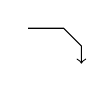
\begin{tikzpicture}[baseline=(O), scale=0.45]
		\coordinate (O) at (0, 0.5);
		\draw[->] (0, 1) -- (1, 1) -- (1.5, 0.5) -- (1.5, 0);
	\end{tikzpicture}$
	memberikan $\identity_{X_1^*}$. Selesailah bukti.
\end{proof}

% segment-id: o014.aljabr2.chapter9.duality-a.p015
Hubungan antara dual kiri dan dual kanan dapat ditulis sebagai
${}^*(X^*)=X$ dan $({}^*X)^*=X$. Walaupun data dualitas sering dipilih dalam
suatu argumen atau uraian, pada hakikatnya dualitas adalah sifat yang dimiliki
sebuah objek, bukan struktur tambahan.

% segment-id: o014.aljabr2.chapter9.duality-a.ex001
\begin{example}
	Dalam setiap kategori monoidal berlaku
	% segment-id: o014.aljabr2.chapter9.duality-a.q005
	\[ \munit^* = \munit = {}^* \munit, \]
	dan morfisme $\mathrm{ev}$ serta $\mathrm{coev}$ yang diperlukan keduanya
	berasal dari kendala unit $\munit\otimes\munit\simeq\munit$.
\end{example}

% segment-id: o014.aljabr2.chapter9.duality-a.d002
\begin{definition}[N.\ Saavedra Rivano]\label{def:rigid-cat}
	\index{kategori monoidal!kaku (rigid)}
	Jika setiap objek dalam kategori monoidal $\mathcal{C}$ memiliki dual kiri
	(atau dual kanan), maka $\mathcal{C}$ disebut kategori \emph{kaku kiri}
	(atau \emph{kaku kanan}).
\end{definition}

% segment-id: o014.aljabr2.chapter9.duality-a.p016
\index{diagram dawai (string diagram)}
Gagasan bukti Definisi--Proposisi~\ref{def:dual-uniqueness} sebenarnya
sederhana, tetapi dalam pelaksanaannya muncul banyak rumus dan diagram
komutatif. Dalam berbagai argumen yang melibatkan dualitas, teknik visualisasi
yang disebut \emph{diagram dawai} sangat berguna; bandingkan
\S\ref{sec:alg-in-monoidal-cat} atau
\cite[Bukti Teorema 2.6.12]{Li1}. Secara terperinci, objek digambarkan sebagai
verteks dan morfisme sebagai anak panah, dengan komposisi dibaca dari atas ke
bawah. Sebagai contoh, $\identity_X$, $f:X\to Y$, $g:Y\to Z$, dan $gf$
masing-masing digambarkan sebagai
% segment-id: o014.aljabr2.chapter9.duality-a.g007
\begin{center}\begin{tikzpicture}[morphism/.style={rectangle, draw, fill=white}]
		\node (A) {$X$};
		\node (B) [below=of A] {$X$};
		\path (A) edge (B);
		
		\node (X) [right=of A] {$X$};
		\node (Y) [below=of X] {$Y$};
		\path (X) edge[->] node[midway, morphism] {$f$} (Y);
		
		\node (Y2) [right=of X] {$Y$};
		\node (Z) [right=of Y] {$Z$};
		\path (Y2) edge[->] node[midway, morphism] {$g$} (Z);
		
		\node (X2) [right=of Y2] {$X$};
		\node (Z2) [below=2cm of X2] {$Z$};
		\path (X2) edge[->] node[near start, morphism] {$f$} node[near end, morphism] {$g$} (Z2);
\end{tikzpicture}\end{center}

% segment-id: o014.aljabr2.chapter9.duality-a.p017
Karena itu, mengomposisikan suatu morfisme dengan $\identity$ di depan atau di
belakang sama dengan memperpanjang anak panahnya. Hasil kali $\otimes$ dari
morfisme-morfisme digambarkan dengan menempatkan anak panahnya berdampingan;
misalnya, $f\otimes g$ digambarkan sebagai
% segment-id: o014.aljabr2.chapter9.duality-a.g008
\begin{center}\begin{tikzpicture}[morphism/.style={rectangle, draw, fill=white}]
		\node (X) {$X$};
		\node (Y) [right=0.1cm of X] {$Y$};
		\node (Y1) [below=of X] {$Y$};
		\node (Z) [below=of Y] {$Z$};
		\path (X) edge[->] node[midway, morphism] {$f$} (Y1);
		\path (Y) edge[->] node[midway, morphism] {$g$} (Z);
\end{tikzpicture}\end{center}

% segment-id: o014.aljabr2.chapter9.duality-a.p018
Karena $X\otimes\munit\simeq X\simeq\munit\otimes X$, unit $\munit$ dapat
dihilangkan dari diagram dawai; dengan kata lain, dawai pada titik tersebut
tidak mempunyai ujung. Jika dualnya ada, morfisme
$\mathrm{ev}:X\otimes X^*\to\munit$ dan
$\mathrm{coev}:\munit\to X^*\otimes X$ dengan demikian masing-masing
digambarkan sebagai
% segment-id: o014.aljabr2.chapter9.duality-a.g009
\begin{center}\begin{tikzpicture}[bend angle=70, auto]
		\node (L) {$X$};
		\node (R) [right=of L] {$X^*$};
		\path (L) edge[bend right] node[midway] {$\mathrm{ev}$} (R);
		
		\node (LL) [right=of R] {$X^*$};
		\node (RR) [right=of LL] {$X$};
		\path (LL) edge[bend left] node[midway] {$\mathrm{coev}$} (RR);
\end{tikzpicture}\end{center}

% segment-id: o014.aljabr2.chapter9.duality-a.p019
Dengan asumsi yang sama, identitas dalam
Definisi~\ref{def:dualizable-obj},
% segment-id: o014.aljabr2.chapter9.duality-a.q006
\[ (\identity_X \otimes \mathrm{ev}) (\mathrm{coev} \otimes \identity_X ) = \identity_X = (\mathrm{ev} \otimes \identity_X) (\identity_X \otimes \mathrm{coev}) \]
digambarkan sebagai
% segment-id: o014.aljabr2.chapter9.duality-a.e001
\begin{equation}\label{eqn:Zorro}
	\begin{tikzpicture}[baseline=(B), bend angle=70, auto]
		\node (A) {$X$};
		\node (B) [below=of A] {$X$};
		\node (C) [left=of B] {${}^* X$};
		\node (D) [left=of C] {$X$};
		\node (E) [below=of D] {$X$};
		
		\path (A) edge (B);
		\path (D) edge[bend left] node {$\mathrm{coev}$} (C);
		\path (C) edge[bend right] node {$\mathrm{ev}$} (B);
		
		\path (D) edge[->] (E);
	\end{tikzpicture} \quad = \quad
	\begin{tikzpicture}[baseline=(M)]
		\node (A) {$X$};
		\node (M) [below=of A] {};
		\node (B) [below=of M] {$X$};
		\path (A) edge (B);
		\coordinate (M) at ($(A)!.5!(B)$);
	\end{tikzpicture} \quad = \quad
	\begin{tikzpicture}[baseline=(B), bend angle=70, auto]
		\node (A) {$X$};
		\node (B) [below=of A] {$X$};
		\node (C) [right=of B] {$X^*$};
		\node (D) [right=of C] {$X$};
		\node (E) [below=of D] {$X$};
		
		\path (A) edge (B);
		\path (C) edge[bend left] node {$\mathrm{coev}$} (D);
		\path (B) edge[bend right] node {$\mathrm{ev}$} (C);
		
		\path (D) edge[->] (E);
	\end{tikzpicture}
\end{equation}
dengan syarat bahwa dual yang dimaksud memang ada. Diagram ini memberi
Definisi~\ref{def:dualizable-obj} nuansa operasional berupa ``meluruskan
dawai''. Dalam sebagian literatur, diagram di atas digambar setelah diputar
sebesar $\frac{\pi}{2}$ dan karena itu juga disebut \emph{identitas Z}.
\index{identitas Z (mark of Zorro)}

% segment-id: o014.aljabr2.chapter9.duality-a.p020
Berdasarkan korespondensi antara identitas aljabar dan operasi pada diagram
dawai ini, identitas aljabar dasar yang melibatkan dualitas mudah ditemukan
dengan mengikuti diagram, atau bahkan dibuktikan langsung melalui diagram.
Sebagai latihan, pembaca dapat mencoba menulis ulang bukti
Definisi--Proposisi~\ref{def:dual-uniqueness} sebagai diagram sederhana.

% segment-id: o014.aljabr2.chapter9.duality-a.p021
Hasil berikut menunjukkan bahwa dualitas secara alami membalik urutan
$\otimes$.

% segment-id: o014.aljabr2.chapter9.duality-a.pr002
\begin{proposition}
	Misalkan $\mathcal{C}$ kategori monoidal dan
	$X,Y\in\Obj(\mathcal{C})$.
	\begin{enumerate}[(i)]
		% segment-id: o014.aljabr2.chapter9.duality-a.i003
		\item Jika $X$ dan $Y$ masing-masing memiliki dual kiri ${}^*X$ dan
		${}^*Y$, maka ${}^*Y\otimes{}^*X$ merupakan dual kiri dari
		$X\otimes Y$. Data yang bersesuaian dapat digambarkan melalui data
		dualitas $X$ dan $Y$ sebagai
		% segment-id: o014.aljabr2.chapter9.duality-a.e002
		\begin{equation*}
			\mathrm{ev}_{X \otimes Y} = \left[ \begin{tikzcd}[column sep=tiny, ampersand replacement=\&]
				{}^* Y \arrow[dash, rrr, bend right=80, "{\mathrm{ev}_Y}"' near end] \& {}^* X \arrow[dash, r, bend right=60, "{\mathrm{ev}_X}"' near start] \& X \& Y
			\end{tikzcd}\right], \quad
			\mathrm{coev}_{X \otimes Y} = \left[ \begin{tikzcd}[column sep=tiny, ampersand replacement=\&]
				X \arrow[dash, rrr, bend left=80, "{\mathrm{coev}_X}" near start] \& Y \arrow[dash, r, bend left=60, "{\mathrm{coev}_Y}" near end] \& {}^* Y \& {}^* X
			\end{tikzcd}\right].
		\end{equation*}
		% segment-id: o014.aljabr2.chapter9.duality-a.i004
		\item Jika $X$ dan $Y$ masing-masing memiliki dual kanan $X^*$ dan
		$Y^*$, maka $Y^*\otimes X^*$ merupakan dual kanan dari $X\otimes Y$.
		Data yang bersesuaian dapat digambarkan melalui data dualitas $X$ dan $Y$
		sebagai
		% segment-id: o014.aljabr2.chapter9.duality-a.e003
		\begin{equation*}
			\mathrm{ev}_{X \otimes Y} = \left[ \begin{tikzcd}[column sep=tiny, ampersand replacement=\&]
				X \arrow[dash, rrr, bend right=80, "{\mathrm{ev}_X}"' near end] \& Y \arrow[dash, r, bend right=60, "{\mathrm{ev}_Y}"' near start] \& Y^* \& X^*
			\end{tikzcd}\right], \quad
			\mathrm{coev}_{X \otimes Y} = \left[ \begin{tikzcd}[column sep=tiny, ampersand replacement=\&]
				X^* \arrow[dash, rrr, bend left=80, "{\mathrm{coev}_X}" near end] \& Y^* \arrow[dash, r, bend left=60, "{\mathrm{coev}_Y}" near start] \& Y \& X
			\end{tikzcd}\right].
		\end{equation*}
	\end{enumerate}
\end{proposition}
% segment-id: o014.aljabr2.chapter9.duality-a.pf003
\begin{proof}
	Kita harus memeriksa identitas dalam
	Definisi~\ref{def:dualizable-obj}, yakni identitas Z
	\eqref{eqn:Zorro}. Hal ini juga ekuivalen dengan memeriksa bahwa
	% segment-id: o014.aljabr2.chapter9.duality-a.q007
	\begin{align*}
		\begin{tikzcd}[column sep=tiny, ampersand replacement=\&]
			{}^* Y \arrow[dash, rrr, bend right=80] \& {}^* X \arrow[dash, r, bend right=60] \& X \arrow[dash, rrr, bend left=80] \& Y \arrow[dash, r, bend left=60] \& {}^* Y \& {}^* X
		\end{tikzcd} & = \begin{tikzcd}[column sep=tiny, ampersand replacement=\&]
			{}^* Y \arrow[dash, d] \& {}^* X \arrow[dash, d] \\
			{}^* Y \& {}^* X 
		\end{tikzcd}, \\
		\begin{tikzcd}[column sep=tiny, ampersand replacement=\&]
			X \arrow[dash, rrr, bend left=80] \& Y \arrow[dash, r, bend left=60] \& {}^* Y \arrow[dash, rrr, bend right=80] \& {}^* X \arrow[dash, r, bend right=60] \& X \& Y
		\end{tikzcd} & = \begin{tikzcd}[column sep=tiny, ampersand replacement=\&]
			X \arrow[dash, d] \& Y \arrow[dash, d] \\
			X \& Y 
		\end{tikzcd}
	\end{align*}
	Tepatnya, diagram-diagram di ruas kiri seharusnya direntangkan ke arah
	vertikal seperti dalam \eqref{eqn:Zorro}, yaitu dengan menyisipkan beberapa
	$\identity$, menggesernya secara horizontal sebagaimana mestinya, lalu
	meluruskannya. Identitas-identitas di atas pun menjadi jelas. Pemeriksaan
	formal yang bersesuaian didasarkan pada berbagai sifat kealamian dari
	kendala unit; rinciannya diserahkan kepada pembaca yang berminat.
\end{proof}

% segment-id: o014.aljabr2.chapter9.duality-a.d003
\begin{definition}\label{def:dual-morphism}
	\index[sym1]{f-star@$f^*, {}^* f$}
	Misalkan $f:X\to Y$ suatu morfisme dalam kategori monoidal $\mathcal{C}$.
	Andaikan $X$ dan $Y$ keduanya memiliki dual kiri ${}^*X$ dan ${}^*Y$
	(atau dual kanan $X^*$ dan $Y^*$). Morfisme dual kiri
	${}^*f:{}^*Y\to{}^*X$ (atau morfisme dual kanan
	$f^*:Y^*\to X^*$) dari $f$ didefinisikan sebagai berikut:
	% segment-id: o014.aljabr2.chapter9.duality-a.e004
	\begin{equation*}\begin{aligned}
		% segment-id: o014.aljabr2.chapter9.duality-a.q008
		{}^* f := (\mathrm{ev}_Y \otimes \identity) (\identity \otimes f \otimes \identity) (\identity \otimes \mathrm{coev}_X) \; &
		\begin{tikzpicture}[baseline=(T), bend angle=70, auto]
			\node (A) {${}^* Y$};
			\node (B) [below=of A] {${}^* Y$};
			\node (C) [right=of B] {$Y$};
			\node (S) [right=of A] {$X$};
			\node[draw, fill=white] (T) at ($(S)!.5!(C)$) {$f$};
			\node (D) [right=of S] {${}^* X$}; 
			\node (E) [below=of D] {${}^* X$};
				
			\path (A) edge (B);
			\path (B) edge[bend right] node {$\mathrm{ev}_Y$} (C);
			\path (C) edge (T);
			\path (T) edge (S);
			\path (S) edge[bend left] node {$\mathrm{coev}_X$} (D);
			\path (D) edge[->] (E);
		\end{tikzpicture}, \\
		% segment-id: o014.aljabr2.chapter9.duality-a.q009
		f^* := (\identity \otimes \mathrm{ev}_Y) (\identity \otimes f \otimes \identity) (\mathrm{coev}_X \otimes \identity) \; &
		\begin{tikzpicture}[baseline=(T), bend angle=70, auto]
			\node (A) {$Y^*$};
			\node (B) [below=of A] {$Y^*$};
			\node (C) [left=of B] {$Y$};
			\node (S) [left=of A] {$X$};
			\node[draw, fill=white] (T) at ($(S)!.5!(C)$) {$f$};
			\node (D) [left=of S] {$X^*$}; 
			\node (E) [below=of D] {$X^*$};
				
			\path (A) edge (B);
			\path (C) edge[bend right] node {$\mathrm{ev}_Y$} (B);
			\path (C) edge (T);
			\path (T) edge (S);
			\path (D) edge[bend left] node {$\mathrm{coev}_X$} (S);
			\path (D) edge[->] (E);
		\end{tikzpicture}.
	\end{aligned}\end{equation*}
\end{definition}
